% Sample Greek scientific book — proof of concept for weebot.
% Build: latexmk -xelatex -shell-escape main.tex
% =====================================================================
% LOCKED Greek scientific-book preamble  (weebot)
% Engine: XeLaTeX (or LuaLaTeX). Do NOT compile with pdfLaTeX.
% Build:  latexmk -xelatex -shell-escape main.tex
%
% This preamble is a *tested, locked* asset. The LLM fills chapter CONTENT
% only; it must never edit this file. See tasks/scientific-book-latex-plan.md.
%
% Load-order note (hard-won): hyperref + bookmark + cleveref are loaded
% BEFORE polyglossia declares Greek. cleveref's polyglossia-Greek language
% hook is broken and throws an "Undefined control sequence" at
% \begin{document}; loading cleveref before the Greek language avoids that
% path, and Greek cross-reference names are supplied manually below. The
% `bookmark` package additionally replaces hyperref's fragile legacy
% begindocument bookmark hook.
% =====================================================================
\documentclass[11pt,a4paper,twoside,openright]{scrbook}

% --- Base font engine ------------------------------------------------
\usepackage{fontspec}

% --- Math ------------------------------------------------------------
\usepackage{amsmath}
\usepackage{amssymb}
\usepackage{mathtools}

% --- Tables ----------------------------------------------------------
\usepackage{booktabs}
\usepackage{longtable}
\usepackage{tabularx}

% --- Figures ---------------------------------------------------------
\usepackage{graphicx}
\usepackage{tikz}
\usepackage{pgfplots}
\pgfplotsset{compat=1.18}
\usepackage{float}
\usepackage[section]{placeins} % \FloatBarrier support for the fixer ladder

% --- Code (minted: needs -shell-escape + Pygments; sandbox-only) -----
\usepackage[newfloat]{minted}
\setminted{fontsize=\small,breaklines=true,tabsize=2}
\usepackage{caption}

% --- Print typography / quality --------------------------------------
\usepackage{microtype}

% --- Cross-references: load BEFORE polyglossia (see load-order note) --
\usepackage[unicode]{hyperref}
\usepackage{bookmark}
\usepackage{cleveref}

% --- Language (Unicode Greek via polyglossia) ------------------------
\usepackage{polyglossia}
\setmainlanguage{greek}
\setotherlanguage{english}

% --- Fonts: GFS Didot (Greek serif) + GFS Neohellenic (Greek sans,
%     used by KOMA headings) + DejaVu mono for code -------------------
\setmainfont{GFS Didot}
\setsansfont{GFS Neohellenic}
\setmonofont{DejaVu Sans Mono}[Scale=0.85]
\newfontfamily\greekfont{GFS Didot}
\newfontfamily\latinfont{GFS Didot}

% --- Bibliography (biblatex + biber): MUST load after polyglossia ----
\usepackage[backend=biber,style=numeric,sorting=nyt]{biblatex}

% --- Greek cross-reference names (cleveref) --------------------------
\crefname{chapter}{κεφάλαιο}{κεφάλαια}
\Crefname{chapter}{Κεφάλαιο}{Κεφάλαια}
\crefname{section}{ενότητα}{ενότητες}
\Crefname{section}{Ενότητα}{Ενότητες}
\crefname{equation}{εξίσωση}{εξισώσεις}
\Crefname{equation}{Εξίσωση}{Εξισώσεις}
\crefname{table}{πίνακας}{πίνακες}
\Crefname{table}{Πίνακας}{Πίνακες}
\crefname{figure}{σχήμα}{σχήματα}
\Crefname{figure}{Σχήμα}{Σχήματα}
\crefname{listing}{κώδικας}{κώδικες}
\Crefname{listing}{Κώδικας}{Κώδικες}


\addbibresource{refs.bib}

\title{Επιστημονικό Εγχειρίδιο: Μαθηματικά, Πληροφορία και Αλγόριθμοι}
\author{weebot}
\date{2026}

\begin{document}

\frontmatter
\maketitle
\tableofcontents

\mainmatter

\chapter{Εισαγωγή στην Ανάλυση}
\label{chap:analysis}

Στο κεφάλαιο αυτό παρουσιάζουμε βασικές έννοιες της μαθηματικής ανάλυσης,
όπως αναπτύχθηκαν ιστορικά από τον Euler \autocite{euler1748}.

\section{Εξισώσεις}
\label{sec:equations}

Η ταυτότητα του Euler συνδέει πέντε θεμελιώδεις σταθερές:
\begin{equation}
  e^{i\pi} + 1 = 0 .
  \label{eq:euler}
\end{equation}

Η \cref{eq:euler} είναι ειδική περίπτωση του τύπου $e^{i\theta} = \cos\theta + i\sin\theta$,
όπου η γωνία $\theta$ (θήτα) μετριέται σε ακτίνια. Ορίζουμε επίσης το άθροισμα
\begin{equation}
  \sum_{\nu=1}^{\infty} \frac{1}{\nu^{2}} = \frac{\pi^{2}}{6},
  \qquad \text{(πρόβλημα της Βασιλείας)} .
\end{equation}

\section{Πίνακες}
\label{sec:tables}

Ο \cref{tab:constants} συνοψίζει μερικές σταθερές.

\begin{table}[htbp]
  \centering
  \caption{Θεμελιώδεις μαθηματικές σταθερές.}
  \label{tab:constants}
  \begin{tabular}{@{}lcl@{}}
    \toprule
    Σταθερά & Σύμβολο & Προσεγγιστική τιμή \\
    \midrule
    Πι            & $\pi$ & $3{,}14159$ \\
    Νεπέριος      & $e$   & $2{,}71828$ \\
    Χρυσή τομή    & $\varphi$ & $1{,}61803$ \\
    \bottomrule
  \end{tabular}
\end{table}

\chapter{Θεωρία Πληροφορίας και Αλγόριθμοι}
\label{chap:information}

\section{Σχήματα}
\label{sec:figures}

Η \cref{fig:entropy} δείχνει τη δυαδική εντροπία \autocite{shannon1948}.

\begin{figure}[htbp]
  \centering
  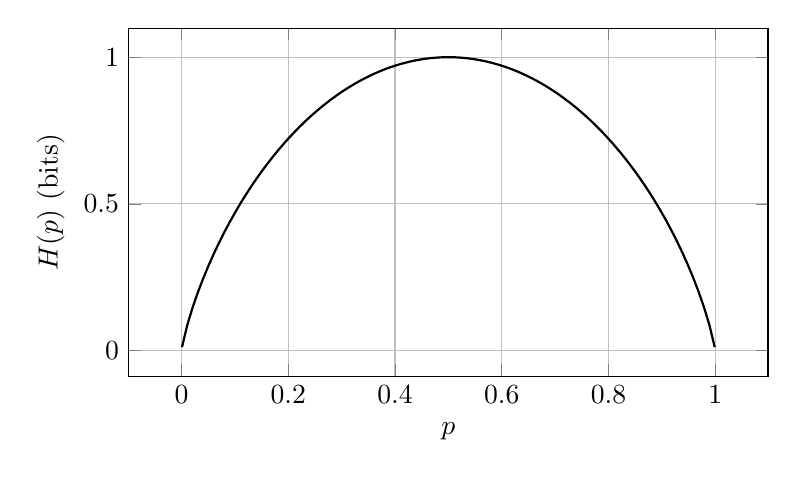
\begin{tikzpicture}
    \begin{axis}[
        width=0.8\linewidth, height=6cm,
        xlabel={$p$}, ylabel={$H(p)$ (bits)},
        domain=0.001:0.999, samples=100, grid=both]
      \addplot[thick] {-x*log2(x) - (1-x)*log2(1-x)};
    \end{axis}
  \end{tikzpicture}
  \caption{Δυαδική συνάρτηση εντροπίας $H(p) = -p\log_2 p - (1-p)\log_2(1-p)$.}
  \label{fig:entropy}
\end{figure}

\section{Κώδικας}
\label{sec:code}

Ο \cref{lst:python} υλοποιεί την εντροπία σε Python, με σχόλια στα Ελληνικά.

\begin{listing}[htbp]
\begin{minted}{python}
import math

def entropy(p: float) -> float:
    # Υπολογίζει τη δυαδική εντροπία για πιθανότητα p
    if p in (0.0, 1.0):
        return 0.0  # οριακή περίπτωση: μηδενική αβεβαιότητα
    return -p * math.log2(p) - (1 - p) * math.log2(1 - p)
\end{minted}
\caption{Συνάρτηση εντροπίας με ελληνικά σχόλια.}
\label{lst:python}
\end{listing}

\backmatter
\printbibliography

\end{document}
